\documentclass[aps,prb,twocolumn,superscriptaddress,amsmath]{revtex4-2}
% \documentclass[aps,prb,twocolumn,superscriptaddress,amsmath]{standalone}

\usepackage{pgfplots}
\usetikzlibrary{arrows.meta}

\pgfplotsset{compat=newest,
   width=7cm,
   height=5cm,
   scale only axis=true,
   max space between ticks=25pt,
   try min ticks=5,
   every axis/.style={
        axis line style={thick,->,>=latex, shorten >=-.4cm}
    },
    every axis plot/.append style={thick},
    tick style={black, thick}
}
\tikzset{
    semithick/.style={line width=0.8pt},
}
\usepgfplotslibrary{groupplots}
\usepgfplotslibrary{dateplot}

\begin{document}
%
% \section{Test section}

% Here is some sample text to fill the column. 

\begin{figure}[h]
    \centering
    % This file was created with tikzplotlib v0.10.1.post13.
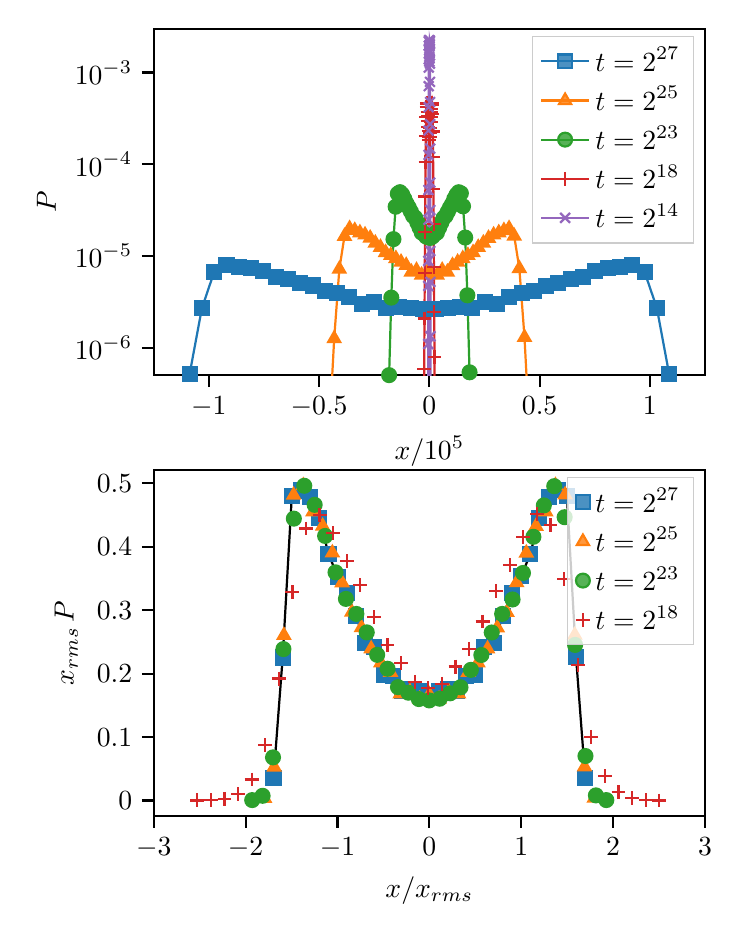
\begin{tikzpicture}

\definecolor{crimson2143940}{RGB}{214,39,40}
\definecolor{darkgrey176}{RGB}{176,176,176}
\definecolor{darkorange25512714}{RGB}{255,127,14}
\definecolor{forestgreen4416044}{RGB}{44,160,44}
\definecolor{lightgrey204}{RGB}{204,204,204}
\definecolor{mediumpurple148103189}{RGB}{148,103,189}
\definecolor{steelblue31119180}{RGB}{31,119,180}

\begin{groupplot}[group style={group size=1 by 2, vertical sep=1.2cm}, height=4.4cm, width=7cm]
\nextgroupplot[
legend cell align={left},
legend style={fill opacity=0.8, draw opacity=1, text opacity=1, draw=lightgrey204},
log basis y={10},
tick align=outside,
tick pos=left,
x grid style={darkgrey176},
xlabel={\(\displaystyle x/10^5\)},
xmin=-1.25, xmax=1.25,
xtick style={color=black},
y grid style={darkgrey176},
ylabel={\(\displaystyle  P \)},
ymin=5e-07, ymax=0.003,
ymode=log,
ytick style={color=black},
ytick={1e-08,1e-07,1e-06,1e-05,0.0001,0.001,0.01,0.1},
yticklabels={
  \(\displaystyle {10^{-8}}\),
  \(\displaystyle {10^{-7}}\),
  \(\displaystyle {10^{-6}}\),
  \(\displaystyle {10^{-5}}\),
  \(\displaystyle {10^{-4}}\),
  \(\displaystyle {10^{-3}}\),
  \(\displaystyle {10^{-2}}\),
  \(\displaystyle {10^{-1}}\)
}
]
\addplot [semithick, steelblue31119180, mark=square*, mark size=2.5, mark options={solid}]
table {%
-1.087597 5.12993007054051e-07
-1.031827 2.6908511793157e-06
-0.976057 6.69963308616709e-06
-0.920287 7.91314924721475e-06
-0.864517 7.55208782423844e-06
-0.808747 7.31456597310671e-06
-0.752977 6.90939757410695e-06
-0.697207 5.87409011714781e-06
-0.641437 5.58457416630147e-06
-0.585667 5.08836711886821e-06
-0.529897 4.76299089648528e-06
-0.474127 4.09943907033615e-06
-0.418357 3.94559325700824e-06
-0.362587 3.60657665362235e-06
-0.306817 3.01039575805922e-06
-0.251047 3.11890252084918e-06
-0.195277 2.67462422863181e-06
-0.139507 2.78678930727756e-06
-0.083737 2.71795786188297e-06
-0.027967 2.6166043926877e-06
0.027803 2.6245277654339e-06
0.083573 2.72068897898097e-06
0.139343 2.78641488348097e-06
0.195113 2.67385380440746e-06
0.250883 3.11896717583025e-06
0.306653 3.00584428823275e-06
0.362423 3.60850964920939e-06
0.418193 3.94454487520201e-06
0.473963 4.09968706691934e-06
0.529733 4.75305517855648e-06
0.585503 5.0923928613821e-06
0.641273 5.58859578417647e-06
0.697043 5.86903759351902e-06
0.752813 6.90479015014643e-06
0.808583 7.30565313207011e-06
0.864353 7.56953810457634e-06
0.920123 7.89292425068137e-06
0.975893 6.70901252080937e-06
1.031663 2.71074093433931e-06
1.087433 5.15831241913013e-07
};
\addlegendentry{\(\displaystyle t=2^{27}\)}
\addplot [semithick, darkorange25512714, mark=triangle*, mark size=2.5, mark options={solid}]
table {%
-0.455096 1.11083707405188e-07
-0.431766 1.25556051680461e-06
-0.408436 7.18106522784207e-06
-0.385106 1.63844933468829e-05
-0.361776 1.98965807334381e-05
-0.338446 1.89886266214221e-05
-0.315116 1.79212053688622e-05
-0.291786 1.69736626358527e-05
-0.268456 1.56507891932657e-05
-0.245126 1.38238284221555e-05
-0.221796 1.24116309324189e-05
-0.198466 1.09143841647616e-05
-0.175136 1.01344561791208e-05
-0.151806 9.37955686050388e-06
-0.128476 8.55686303167119e-06
-0.105146 7.89660524401105e-06
-0.081816 6.68761647354384e-06
-0.058486 6.97712243822927e-06
-0.035156 6.1971734841644e-06
-0.011826 6.52359354705434e-06
0.011504 6.52782188981759e-06
0.034834 6.19943137991142e-06
0.058164 6.98637137410106e-06
0.081494 6.67149742194123e-06
0.104824 7.87887745663666e-06
0.128154 8.5581390379578e-06
0.151484 9.3599827538696e-06
0.174814 1.01342029413964e-05
0.198144 1.0878780997833e-05
0.221474 1.24083791080392e-05
0.244804 1.38444233948897e-05
0.268134 1.55779830937753e-05
0.291464 1.69627378735057e-05
0.314794 1.79242471291137e-05
0.338124 1.89364013782921e-05
0.361454 1.99361470841073e-05
0.384784 1.64797543174025e-05
0.408114 7.29544742560842e-06
0.431444 1.29571119846365e-06
0.454774 1.10816066526556e-07
};
\addlegendentry{\(\displaystyle t=2^{25}\)}
\addplot [semithick, forestgreen4416044, mark=*, mark size=2.5, mark options={solid}]
table {%
-0.192429 8.23823568211934e-08
-0.182569 5.01038415322224e-07
-0.172709 3.51121303646045e-06
-0.162849 1.52473351033356e-05
-0.152989 3.44092503127113e-05
-0.143129 4.77273125822628e-05
-0.133269 4.95885461691458e-05
-0.123409 4.68109683276989e-05
-0.113549 4.20019541931485e-05
-0.103689 3.72489056761325e-05
-0.093829 3.38497266199008e-05
-0.083969 3.04773167077981e-05
-0.074109 2.73360496326347e-05
-0.064249 2.60775319112013e-05
-0.054389 2.30755753442641e-05
-0.044529 2.03725351470588e-05
-0.034669 1.79514526941064e-05
-0.024809 1.74886116090264e-05
-0.014949 1.6282976870746e-05
-0.005089 1.59321578513635e-05
0.004771 1.57313423974532e-05
0.014631 1.62886010864323e-05
0.024491 1.74322948493915e-05
0.034351 1.79341307716362e-05
0.044211 2.03192508040343e-05
0.054071 2.30359526070543e-05
0.063931 2.5828894579671e-05
0.073791 2.73647030183683e-05
0.083651 3.03802578273608e-05
0.093511 3.37490886516791e-05
0.103371 3.69615946123507e-05
0.113231 4.20557869461348e-05
0.123091 4.64876207713545e-05
0.132951 4.95391557274059e-05
0.142811 4.82374508812261e-05
0.152671 3.47763816818797e-05
0.162531 1.58738139053414e-05
0.172391 3.72443383744084e-06
0.182251 5.38237597551207e-07
0.192111 7.98606241731395e-08
};
\addlegendentry{\(\displaystyle t=2^{23}\)}
\addplot [semithick, crimson2143940, mark=+, mark size=2.5, mark options={solid}]
table {%
-0.024688 1.8908489760873e-07
-0.023428 5.90274120130556e-07
-0.022168 2.07923150050397e-06
-0.020908 6.58005891473968e-06
-0.019648 1.83707262811508e-05
-0.018388 4.45365892742063e-05
-0.017128 0.000105986356805556
-0.015868 0.00020458834565873
-0.014608 0.000330280127142857
-0.013348 0.000423118224722222
-0.012088 0.000462105562896825
-0.010828 0.000452517540436508
-0.009568 0.000417412210952381
-0.008308 0.000372279224722222
-0.007048 0.000338633175238095
-0.005788 0.000294731150833333
-0.004528 0.000253131794960317
-0.003268 0.000228899158412698
-0.002008 0.000196763061309524
-0.000748 0.000185201958730159
0.000512 0.000184293000912698
0.001772 0.000196943668849206
0.003032 0.000220727737539683
0.004292 0.000248173976984127
0.005552 0.000287749479126984
0.006812 0.000329263664047619
0.008072 0.000369707439642857
0.009332 0.00040424656047619
0.010592 0.000444381415873016
0.011852 0.000466213856666667
0.013112 0.000438252085793651
0.014372 0.000349982778611111
0.015632 0.000227399124206349
0.016892 0.000120876504916667
0.018152 5.3342174440873e-05
0.019412 2.23723494702381e-05
0.020672 7.5197180770119e-06
0.021932 2.42717042334683e-06
0.023192 7.87495928734921e-07
0.024452 1.89082405790079e-07
};
\addlegendentry{\(\displaystyle t=2^{18}\)}
\addplot [semithick, mediumpurple148103189, mark=x, mark size=2.5, mark options={solid}]
table {%
-0.005834 2.738438295e-07
-0.005544 0
-0.005254 1.09538580185172e-06
-0.004964 4.70281556743104e-06
-0.004674 8.8391987412069e-06
-0.004384 2.47983698965517e-05
-0.004094 5.23101797931034e-05
-0.003804 0.000126398901931034
-0.003514 0.000232931472758621
-0.003224 0.000419123161206897
-0.002934 0.000709943868448276
-0.002644 0.00113378345913793
-0.002354 0.00160075111896552
-0.002064 0.00195556481034483
-0.001774 0.00219713176551724
-0.001484 0.00225409588103448
-0.001194 0.00218915992931034
-0.000904 0.00197591668793103
-0.000614 0.00174597121034483
-0.000324 0.00147793051034483
-3.4e-05 0.0013150636137931
0.000256 0.00142612189827586
0.000546 0.00167460211206897
0.000836 0.00191692699137931
0.001126 0.0021582397637931
0.001416 0.00224817453103448
0.001706 0.00222905264137931
0.001996 0.00203512883793104
0.002286 0.00168717621724138
0.002576 0.00125053118948276
0.002866 0.000791999054137931
0.003156 0.000477260349310345
0.003446 0.000273930857586207
0.003736 0.000148269580034483
0.004026 6.30957925517241e-05
0.004316 3.16583332448276e-05
0.004606 1.13126185377586e-05
0.004896 5.20105582967241e-06
0.005186 1.33101979336897e-06
0.005476 2.72952429e-07
0.005766 5.58589568965517e-10
};
\addlegendentry{\(\displaystyle t=2^{14}\)}

\nextgroupplot[
legend cell align={left},
legend style={fill opacity=0.8, draw opacity=1, text opacity=1, draw=lightgrey204},
tick align=outside,
tick pos=left,
x grid style={darkgrey176},
xlabel={\(\displaystyle x / x_{rms}\)},
xmin=-3, xmax=3,
xtick style={color=black},
y grid style={darkgrey176},
ylabel={\(\displaystyle  x_{rms} \, P\)},
ymin=-0.0245997307740645, ymax=0.521320073709912,
ytick style={color=black}
]
\addplot [semithick, black, forget plot]
table {%
-1.69685345800962 0.0351235244635792
-1.59704149633558 0.225429907601863
-1.49722953466153 0.48036746024812
-1.39741757298749 0.488597688664373
-1.29760561131345 0.477770823340559
-1.1977936496394 0.444548663763906
-1.09798168796536 0.388692627824925
-0.998169726291318 0.352947789429801
-0.898357764617275 0.326597416779799
-0.798545802943232 0.290410544989811
-0.698733841269189 0.248381846547796
-0.598921879595146 0.242503314666908
-0.499109917921103 0.198441906687418
-0.39929795624706 0.196710504395756
-0.299485994573017 0.172163219500433
-0.199674032898974 0.17594891984523
-0.0998620712249305 0.172411963214107
-5.0109550887502e-05 0.165901338328916
0.0997618521231555 0.17257703184217
0.199573813797199 0.17589495275514
0.299385775471242 0.172143760978677
0.399197737145285 0.196607611768738
0.499009698819328 0.198445605763933
0.598821660493371 0.242613607939698
0.698633622167414 0.248213401716399
0.798445583841457 0.290410001323135
0.8982575455155 0.326503082035365
0.998069507189543 0.353117755126006
1.09788146886359 0.388257576147144
1.19769343053763 0.444728942001085
1.29750539221167 0.477668502530443
1.39731735388571 0.488708239394337
1.49712931555976 0.480487792614644
1.5969412772338 0.225567138013743
1.69675323890784 0.035323198529156
};
\addplot [semithick, steelblue31119180, mark=square*, mark size=2.5, mark options={solid}, only marks]
table {%
-1.69685345800962 0.0351235244635792
-1.59704149633558 0.225429907601863
-1.49722953466153 0.48036746024812
-1.39741757298749 0.488597688664373
-1.29760561131345 0.477770823340559
-1.1977936496394 0.444548663763906
-1.09798168796536 0.388692627824925
-0.998169726291318 0.352947789429801
-0.898357764617275 0.326597416779799
-0.798545802943232 0.290410544989811
-0.698733841269189 0.248381846547796
-0.598921879595146 0.242503314666908
-0.499109917921103 0.198441906687418
-0.39929795624706 0.196710504395756
-0.299485994573017 0.172163219500433
-0.199674032898974 0.17594891984523
-0.0998620712249305 0.172411963214107
-5.0109550887502e-05 0.165901338328916
0.0997618521231555 0.17257703184217
0.199573813797199 0.17589495275514
0.299385775471242 0.172143760978677
0.399197737145285 0.196607611768738
0.499009698819328 0.198445605763933
0.598821660493371 0.242613607939698
0.698633622167414 0.248213401716399
0.798445583841457 0.290410001323135
0.8982575455155 0.326503082035365
0.998069507189543 0.353117755126006
1.09788146886359 0.388257576147144
1.19769343053763 0.444728942001085
1.29750539221167 0.477668502530443
1.39731735388571 0.488708239394337
1.49712931555976 0.480487792614644
1.5969412772338 0.225567138013743
1.69675323890784 0.035323198529156
};
\addlegendentry{\(\displaystyle t=2^{27}\)}
\addplot [semithick, darkorange25512714, mark=triangle*, mark size=2.5, mark options={solid}, only marks]
table {%
-1.79491129727995 0.00373426957431449
-1.68933666261309 0.0528518213586198
-1.58376202794623 0.26039060257673
-1.47818739327937 0.481370345570397
-1.37261275861251 0.49632245900742
-1.26703812394565 0.45498231495888
-1.16146348927878 0.432500590197787
-1.05588885461192 0.390322564065994
-0.950314219945061 0.343317225931999
-0.844739585278199 0.296865824135353
-0.739164950611338 0.272514334123349
-0.633590315944476 0.239199172506601
-0.528015681277615 0.217085812835817
-0.422441046610753 0.202259007205263
-0.316866411943892 0.168102247382213
-0.21129177727703 0.17154692580208
-0.105717142610169 0.160059486425459
-0.00014250794330735 0.167062748995738
0.105432126723554 0.160023172747558
0.211006761390416 0.171445797621472
0.316581396057277 0.168148231513764
0.422156030724139 0.202133631521589
0.527730665391 0.217190087192492
0.633305300057862 0.239092340538529
0.738879934724723 0.272307668594877
0.844454569391585 0.296696671014954
0.950029204058446 0.343407906678343
1.05560383872531 0.390152553442694
1.16117847339217 0.432254751838205
1.26675310805903 0.454995591032921
1.37232774272589 0.496505537142458
1.47790237739275 0.48179396889123
1.58347701205962 0.260809953465067
1.68905164672648 0.0531457966287965
1.79462628139334 0.00377848313082298
};
\addlegendentry{\(\displaystyle t=2^{25}\)}
\addplot [semithick, forestgreen4416044, mark=*, mark size=2.5, mark options={solid}, only marks]
table {%
-1.92882947091101 0.000761245918001764
-1.81544821380617 0.00751092501997092
-1.70206695670134 0.0680527199535696
-1.58868569959651 0.23871574219349
-1.47530444249167 0.444207206253079
-1.36192318538684 0.495996701094989
-1.24854192828201 0.465962816612787
-1.13516067117717 0.416946371471856
-1.02177941407234 0.359665731441207
-0.908398156967507 0.317781641359896
-0.795016899862674 0.294098305911668
-0.681635642757841 0.26505080925513
-0.568254385653008 0.229635198526429
-0.454873128548174 0.207694134704626
-0.341491871443341 0.178787094407612
-0.228110614338508 0.169951077773474
-0.114729357233675 0.159967304699489
-0.00134810012884185 0.157835521694817
0.112033156975991 0.160482453257572
0.225414414080824 0.16903255328075
0.338795671185658 0.17853657247977
0.452176928290491 0.205978231898554
0.565558185395324 0.22935949844142
0.678939442500157 0.264836626260142
0.79232069960499 0.294117955215571
0.905701956709823 0.316870598213437
1.01908321381466 0.358607867511269
1.13246447091949 0.415629664490562
1.24584572802432 0.465078502320713
1.35922698512916 0.495389159596087
1.47260824223399 0.446519517829329
1.58598949933882 0.245220510006179
1.69937075644366 0.0701814471322813
1.81275201354849 0.00815175645216166
1.92613327065332 0.000783467580405326
};
\addlegendentry{\(\displaystyle t=2^{23}\)}
\addplot [semithick, crimson2143940, mark=+, mark size=2.5, mark options={solid}, only marks]
table {%
-2.52611181327276 0.000268508664361216
-2.37822983054601 0.00080552352141304
-2.23034784781925 0.00288791186142534
-2.08246586509249 0.00974844376405332
-1.93458388236573 0.0330928857073305
-1.78670189963898 0.0872414495472249
-1.63881991691222 0.192215469077943
-1.49093793418546 0.328408149116685
-1.3430559514587 0.42859424340496
-1.19517396873195 0.450335898140147
-1.04729198600519 0.421096069830639
-0.899410003278432 0.377182877768568
-0.751528020551674 0.339406818021506
-0.603646037824917 0.288668853114288
-0.455764055098159 0.244649791596646
-0.307882072371402 0.216811954362569
-0.160000089644645 0.187179778730351
-0.0121181069178871 0.177816937466866
0.13576387580887 0.183953410201863
0.283645858535628 0.211106190587688
0.431527841262385 0.2389771582269
0.579409823989143 0.282220741942003
0.7272918067159 0.33043246972343
0.875173789442658 0.37104290656817
1.02305577216942 0.414874992739051
1.17093775489617 0.451069233892078
1.31881973762293 0.434181172689825
1.46670172034969 0.348780846381413
1.61458370307644 0.21360157104713
1.7624656858032 0.10032746783233
1.91034766852996 0.0386424674235587
2.05822965125672 0.0129490578789015
2.20611163398347 0.00396519305146631
2.35399361671023 0.000859224535363965
2.50187559943699 0.000214805793388936
};
\addlegendentry{\(\displaystyle t=2^{18}\)}
\end{groupplot}

\end{tikzpicture}

    \caption{Here is sample caption to match to the figure text size to the caption text size.}
\end{figure}

% \vfill\null

\newpage

\begin{figure}
    \centering
    % This file was created with tikzplotlib v0.10.1.post13.
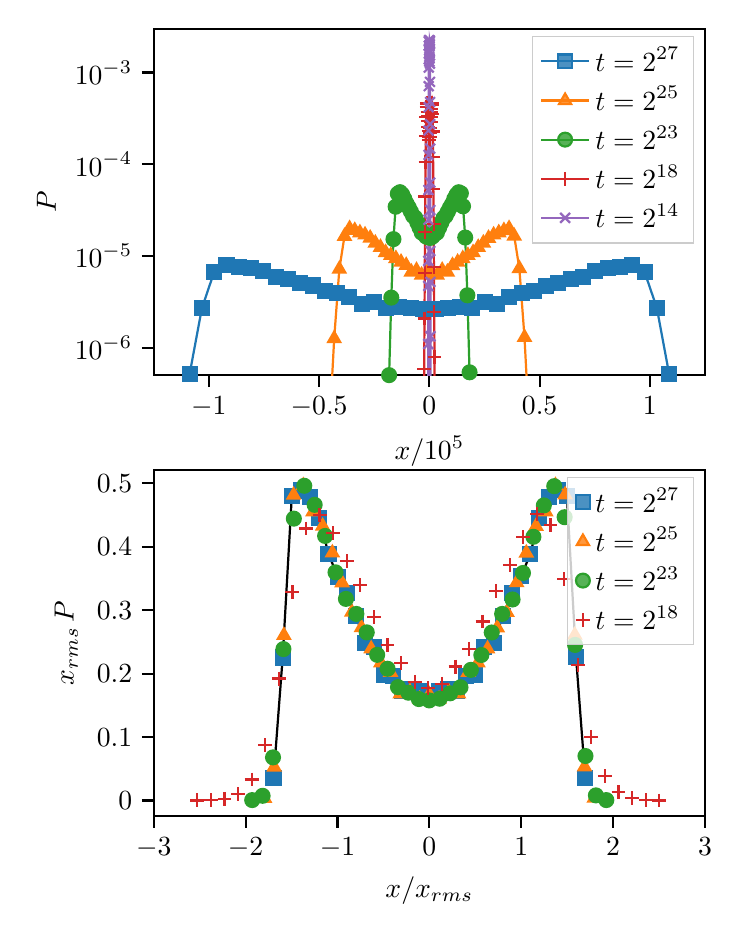
\begin{tikzpicture}

\definecolor{crimson2143940}{RGB}{214,39,40}
\definecolor{darkgrey176}{RGB}{176,176,176}
\definecolor{darkorange25512714}{RGB}{255,127,14}
\definecolor{forestgreen4416044}{RGB}{44,160,44}
\definecolor{lightgrey204}{RGB}{204,204,204}
\definecolor{mediumpurple148103189}{RGB}{148,103,189}
\definecolor{steelblue31119180}{RGB}{31,119,180}

\begin{groupplot}[group style={group size=1 by 2, vertical sep=1.2cm}, height=4.4cm, width=7cm]
\nextgroupplot[
legend cell align={left},
legend style={fill opacity=0.8, draw opacity=1, text opacity=1, draw=lightgrey204},
log basis y={10},
tick align=outside,
tick pos=left,
x grid style={darkgrey176},
xlabel={\(\displaystyle x/10^5\)},
xmin=-1.25, xmax=1.25,
xtick style={color=black},
y grid style={darkgrey176},
ylabel={\(\displaystyle  P \)},
ymin=5e-07, ymax=0.003,
ymode=log,
ytick style={color=black},
ytick={1e-08,1e-07,1e-06,1e-05,0.0001,0.001,0.01,0.1},
yticklabels={
  \(\displaystyle {10^{-8}}\),
  \(\displaystyle {10^{-7}}\),
  \(\displaystyle {10^{-6}}\),
  \(\displaystyle {10^{-5}}\),
  \(\displaystyle {10^{-4}}\),
  \(\displaystyle {10^{-3}}\),
  \(\displaystyle {10^{-2}}\),
  \(\displaystyle {10^{-1}}\)
}
]
\addplot [semithick, steelblue31119180, mark=square*, mark size=2.5, mark options={solid}]
table {%
-1.087597 5.12993007054051e-07
-1.031827 2.6908511793157e-06
-0.976057 6.69963308616709e-06
-0.920287 7.91314924721475e-06
-0.864517 7.55208782423844e-06
-0.808747 7.31456597310671e-06
-0.752977 6.90939757410695e-06
-0.697207 5.87409011714781e-06
-0.641437 5.58457416630147e-06
-0.585667 5.08836711886821e-06
-0.529897 4.76299089648528e-06
-0.474127 4.09943907033615e-06
-0.418357 3.94559325700824e-06
-0.362587 3.60657665362235e-06
-0.306817 3.01039575805922e-06
-0.251047 3.11890252084918e-06
-0.195277 2.67462422863181e-06
-0.139507 2.78678930727756e-06
-0.083737 2.71795786188297e-06
-0.027967 2.6166043926877e-06
0.027803 2.6245277654339e-06
0.083573 2.72068897898097e-06
0.139343 2.78641488348097e-06
0.195113 2.67385380440746e-06
0.250883 3.11896717583025e-06
0.306653 3.00584428823275e-06
0.362423 3.60850964920939e-06
0.418193 3.94454487520201e-06
0.473963 4.09968706691934e-06
0.529733 4.75305517855648e-06
0.585503 5.0923928613821e-06
0.641273 5.58859578417647e-06
0.697043 5.86903759351902e-06
0.752813 6.90479015014643e-06
0.808583 7.30565313207011e-06
0.864353 7.56953810457634e-06
0.920123 7.89292425068137e-06
0.975893 6.70901252080937e-06
1.031663 2.71074093433931e-06
1.087433 5.15831241913013e-07
};
\addlegendentry{\(\displaystyle t=2^{27}\)}
\addplot [semithick, darkorange25512714, mark=triangle*, mark size=2.5, mark options={solid}]
table {%
-0.455096 1.11083707405188e-07
-0.431766 1.25556051680461e-06
-0.408436 7.18106522784207e-06
-0.385106 1.63844933468829e-05
-0.361776 1.98965807334381e-05
-0.338446 1.89886266214221e-05
-0.315116 1.79212053688622e-05
-0.291786 1.69736626358527e-05
-0.268456 1.56507891932657e-05
-0.245126 1.38238284221555e-05
-0.221796 1.24116309324189e-05
-0.198466 1.09143841647616e-05
-0.175136 1.01344561791208e-05
-0.151806 9.37955686050388e-06
-0.128476 8.55686303167119e-06
-0.105146 7.89660524401105e-06
-0.081816 6.68761647354384e-06
-0.058486 6.97712243822927e-06
-0.035156 6.1971734841644e-06
-0.011826 6.52359354705434e-06
0.011504 6.52782188981759e-06
0.034834 6.19943137991142e-06
0.058164 6.98637137410106e-06
0.081494 6.67149742194123e-06
0.104824 7.87887745663666e-06
0.128154 8.5581390379578e-06
0.151484 9.3599827538696e-06
0.174814 1.01342029413964e-05
0.198144 1.0878780997833e-05
0.221474 1.24083791080392e-05
0.244804 1.38444233948897e-05
0.268134 1.55779830937753e-05
0.291464 1.69627378735057e-05
0.314794 1.79242471291137e-05
0.338124 1.89364013782921e-05
0.361454 1.99361470841073e-05
0.384784 1.64797543174025e-05
0.408114 7.29544742560842e-06
0.431444 1.29571119846365e-06
0.454774 1.10816066526556e-07
};
\addlegendentry{\(\displaystyle t=2^{25}\)}
\addplot [semithick, forestgreen4416044, mark=*, mark size=2.5, mark options={solid}]
table {%
-0.192429 8.23823568211934e-08
-0.182569 5.01038415322224e-07
-0.172709 3.51121303646045e-06
-0.162849 1.52473351033356e-05
-0.152989 3.44092503127113e-05
-0.143129 4.77273125822628e-05
-0.133269 4.95885461691458e-05
-0.123409 4.68109683276989e-05
-0.113549 4.20019541931485e-05
-0.103689 3.72489056761325e-05
-0.093829 3.38497266199008e-05
-0.083969 3.04773167077981e-05
-0.074109 2.73360496326347e-05
-0.064249 2.60775319112013e-05
-0.054389 2.30755753442641e-05
-0.044529 2.03725351470588e-05
-0.034669 1.79514526941064e-05
-0.024809 1.74886116090264e-05
-0.014949 1.6282976870746e-05
-0.005089 1.59321578513635e-05
0.004771 1.57313423974532e-05
0.014631 1.62886010864323e-05
0.024491 1.74322948493915e-05
0.034351 1.79341307716362e-05
0.044211 2.03192508040343e-05
0.054071 2.30359526070543e-05
0.063931 2.5828894579671e-05
0.073791 2.73647030183683e-05
0.083651 3.03802578273608e-05
0.093511 3.37490886516791e-05
0.103371 3.69615946123507e-05
0.113231 4.20557869461348e-05
0.123091 4.64876207713545e-05
0.132951 4.95391557274059e-05
0.142811 4.82374508812261e-05
0.152671 3.47763816818797e-05
0.162531 1.58738139053414e-05
0.172391 3.72443383744084e-06
0.182251 5.38237597551207e-07
0.192111 7.98606241731395e-08
};
\addlegendentry{\(\displaystyle t=2^{23}\)}
\addplot [semithick, crimson2143940, mark=+, mark size=2.5, mark options={solid}]
table {%
-0.024688 1.8908489760873e-07
-0.023428 5.90274120130556e-07
-0.022168 2.07923150050397e-06
-0.020908 6.58005891473968e-06
-0.019648 1.83707262811508e-05
-0.018388 4.45365892742063e-05
-0.017128 0.000105986356805556
-0.015868 0.00020458834565873
-0.014608 0.000330280127142857
-0.013348 0.000423118224722222
-0.012088 0.000462105562896825
-0.010828 0.000452517540436508
-0.009568 0.000417412210952381
-0.008308 0.000372279224722222
-0.007048 0.000338633175238095
-0.005788 0.000294731150833333
-0.004528 0.000253131794960317
-0.003268 0.000228899158412698
-0.002008 0.000196763061309524
-0.000748 0.000185201958730159
0.000512 0.000184293000912698
0.001772 0.000196943668849206
0.003032 0.000220727737539683
0.004292 0.000248173976984127
0.005552 0.000287749479126984
0.006812 0.000329263664047619
0.008072 0.000369707439642857
0.009332 0.00040424656047619
0.010592 0.000444381415873016
0.011852 0.000466213856666667
0.013112 0.000438252085793651
0.014372 0.000349982778611111
0.015632 0.000227399124206349
0.016892 0.000120876504916667
0.018152 5.3342174440873e-05
0.019412 2.23723494702381e-05
0.020672 7.5197180770119e-06
0.021932 2.42717042334683e-06
0.023192 7.87495928734921e-07
0.024452 1.89082405790079e-07
};
\addlegendentry{\(\displaystyle t=2^{18}\)}
\addplot [semithick, mediumpurple148103189, mark=x, mark size=2.5, mark options={solid}]
table {%
-0.005834 2.738438295e-07
-0.005544 0
-0.005254 1.09538580185172e-06
-0.004964 4.70281556743104e-06
-0.004674 8.8391987412069e-06
-0.004384 2.47983698965517e-05
-0.004094 5.23101797931034e-05
-0.003804 0.000126398901931034
-0.003514 0.000232931472758621
-0.003224 0.000419123161206897
-0.002934 0.000709943868448276
-0.002644 0.00113378345913793
-0.002354 0.00160075111896552
-0.002064 0.00195556481034483
-0.001774 0.00219713176551724
-0.001484 0.00225409588103448
-0.001194 0.00218915992931034
-0.000904 0.00197591668793103
-0.000614 0.00174597121034483
-0.000324 0.00147793051034483
-3.4e-05 0.0013150636137931
0.000256 0.00142612189827586
0.000546 0.00167460211206897
0.000836 0.00191692699137931
0.001126 0.0021582397637931
0.001416 0.00224817453103448
0.001706 0.00222905264137931
0.001996 0.00203512883793104
0.002286 0.00168717621724138
0.002576 0.00125053118948276
0.002866 0.000791999054137931
0.003156 0.000477260349310345
0.003446 0.000273930857586207
0.003736 0.000148269580034483
0.004026 6.30957925517241e-05
0.004316 3.16583332448276e-05
0.004606 1.13126185377586e-05
0.004896 5.20105582967241e-06
0.005186 1.33101979336897e-06
0.005476 2.72952429e-07
0.005766 5.58589568965517e-10
};
\addlegendentry{\(\displaystyle t=2^{14}\)}

\nextgroupplot[
legend cell align={left},
legend style={fill opacity=0.8, draw opacity=1, text opacity=1, draw=lightgrey204},
tick align=outside,
tick pos=left,
x grid style={darkgrey176},
xlabel={\(\displaystyle x / x_{rms}\)},
xmin=-3, xmax=3,
xtick style={color=black},
y grid style={darkgrey176},
ylabel={\(\displaystyle  x_{rms} \, P\)},
ymin=-0.0245997307740645, ymax=0.521320073709912,
ytick style={color=black}
]
\addplot [semithick, black, forget plot]
table {%
-1.69685345800962 0.0351235244635792
-1.59704149633558 0.225429907601863
-1.49722953466153 0.48036746024812
-1.39741757298749 0.488597688664373
-1.29760561131345 0.477770823340559
-1.1977936496394 0.444548663763906
-1.09798168796536 0.388692627824925
-0.998169726291318 0.352947789429801
-0.898357764617275 0.326597416779799
-0.798545802943232 0.290410544989811
-0.698733841269189 0.248381846547796
-0.598921879595146 0.242503314666908
-0.499109917921103 0.198441906687418
-0.39929795624706 0.196710504395756
-0.299485994573017 0.172163219500433
-0.199674032898974 0.17594891984523
-0.0998620712249305 0.172411963214107
-5.0109550887502e-05 0.165901338328916
0.0997618521231555 0.17257703184217
0.199573813797199 0.17589495275514
0.299385775471242 0.172143760978677
0.399197737145285 0.196607611768738
0.499009698819328 0.198445605763933
0.598821660493371 0.242613607939698
0.698633622167414 0.248213401716399
0.798445583841457 0.290410001323135
0.8982575455155 0.326503082035365
0.998069507189543 0.353117755126006
1.09788146886359 0.388257576147144
1.19769343053763 0.444728942001085
1.29750539221167 0.477668502530443
1.39731735388571 0.488708239394337
1.49712931555976 0.480487792614644
1.5969412772338 0.225567138013743
1.69675323890784 0.035323198529156
};
\addplot [semithick, steelblue31119180, mark=square*, mark size=2.5, mark options={solid}, only marks]
table {%
-1.69685345800962 0.0351235244635792
-1.59704149633558 0.225429907601863
-1.49722953466153 0.48036746024812
-1.39741757298749 0.488597688664373
-1.29760561131345 0.477770823340559
-1.1977936496394 0.444548663763906
-1.09798168796536 0.388692627824925
-0.998169726291318 0.352947789429801
-0.898357764617275 0.326597416779799
-0.798545802943232 0.290410544989811
-0.698733841269189 0.248381846547796
-0.598921879595146 0.242503314666908
-0.499109917921103 0.198441906687418
-0.39929795624706 0.196710504395756
-0.299485994573017 0.172163219500433
-0.199674032898974 0.17594891984523
-0.0998620712249305 0.172411963214107
-5.0109550887502e-05 0.165901338328916
0.0997618521231555 0.17257703184217
0.199573813797199 0.17589495275514
0.299385775471242 0.172143760978677
0.399197737145285 0.196607611768738
0.499009698819328 0.198445605763933
0.598821660493371 0.242613607939698
0.698633622167414 0.248213401716399
0.798445583841457 0.290410001323135
0.8982575455155 0.326503082035365
0.998069507189543 0.353117755126006
1.09788146886359 0.388257576147144
1.19769343053763 0.444728942001085
1.29750539221167 0.477668502530443
1.39731735388571 0.488708239394337
1.49712931555976 0.480487792614644
1.5969412772338 0.225567138013743
1.69675323890784 0.035323198529156
};
\addlegendentry{\(\displaystyle t=2^{27}\)}
\addplot [semithick, darkorange25512714, mark=triangle*, mark size=2.5, mark options={solid}, only marks]
table {%
-1.79491129727995 0.00373426957431449
-1.68933666261309 0.0528518213586198
-1.58376202794623 0.26039060257673
-1.47818739327937 0.481370345570397
-1.37261275861251 0.49632245900742
-1.26703812394565 0.45498231495888
-1.16146348927878 0.432500590197787
-1.05588885461192 0.390322564065994
-0.950314219945061 0.343317225931999
-0.844739585278199 0.296865824135353
-0.739164950611338 0.272514334123349
-0.633590315944476 0.239199172506601
-0.528015681277615 0.217085812835817
-0.422441046610753 0.202259007205263
-0.316866411943892 0.168102247382213
-0.21129177727703 0.17154692580208
-0.105717142610169 0.160059486425459
-0.00014250794330735 0.167062748995738
0.105432126723554 0.160023172747558
0.211006761390416 0.171445797621472
0.316581396057277 0.168148231513764
0.422156030724139 0.202133631521589
0.527730665391 0.217190087192492
0.633305300057862 0.239092340538529
0.738879934724723 0.272307668594877
0.844454569391585 0.296696671014954
0.950029204058446 0.343407906678343
1.05560383872531 0.390152553442694
1.16117847339217 0.432254751838205
1.26675310805903 0.454995591032921
1.37232774272589 0.496505537142458
1.47790237739275 0.48179396889123
1.58347701205962 0.260809953465067
1.68905164672648 0.0531457966287965
1.79462628139334 0.00377848313082298
};
\addlegendentry{\(\displaystyle t=2^{25}\)}
\addplot [semithick, forestgreen4416044, mark=*, mark size=2.5, mark options={solid}, only marks]
table {%
-1.92882947091101 0.000761245918001764
-1.81544821380617 0.00751092501997092
-1.70206695670134 0.0680527199535696
-1.58868569959651 0.23871574219349
-1.47530444249167 0.444207206253079
-1.36192318538684 0.495996701094989
-1.24854192828201 0.465962816612787
-1.13516067117717 0.416946371471856
-1.02177941407234 0.359665731441207
-0.908398156967507 0.317781641359896
-0.795016899862674 0.294098305911668
-0.681635642757841 0.26505080925513
-0.568254385653008 0.229635198526429
-0.454873128548174 0.207694134704626
-0.341491871443341 0.178787094407612
-0.228110614338508 0.169951077773474
-0.114729357233675 0.159967304699489
-0.00134810012884185 0.157835521694817
0.112033156975991 0.160482453257572
0.225414414080824 0.16903255328075
0.338795671185658 0.17853657247977
0.452176928290491 0.205978231898554
0.565558185395324 0.22935949844142
0.678939442500157 0.264836626260142
0.79232069960499 0.294117955215571
0.905701956709823 0.316870598213437
1.01908321381466 0.358607867511269
1.13246447091949 0.415629664490562
1.24584572802432 0.465078502320713
1.35922698512916 0.495389159596087
1.47260824223399 0.446519517829329
1.58598949933882 0.245220510006179
1.69937075644366 0.0701814471322813
1.81275201354849 0.00815175645216166
1.92613327065332 0.000783467580405326
};
\addlegendentry{\(\displaystyle t=2^{23}\)}
\addplot [semithick, crimson2143940, mark=+, mark size=2.5, mark options={solid}, only marks]
table {%
-2.52611181327276 0.000268508664361216
-2.37822983054601 0.00080552352141304
-2.23034784781925 0.00288791186142534
-2.08246586509249 0.00974844376405332
-1.93458388236573 0.0330928857073305
-1.78670189963898 0.0872414495472249
-1.63881991691222 0.192215469077943
-1.49093793418546 0.328408149116685
-1.3430559514587 0.42859424340496
-1.19517396873195 0.450335898140147
-1.04729198600519 0.421096069830639
-0.899410003278432 0.377182877768568
-0.751528020551674 0.339406818021506
-0.603646037824917 0.288668853114288
-0.455764055098159 0.244649791596646
-0.307882072371402 0.216811954362569
-0.160000089644645 0.187179778730351
-0.0121181069178871 0.177816937466866
0.13576387580887 0.183953410201863
0.283645858535628 0.211106190587688
0.431527841262385 0.2389771582269
0.579409823989143 0.282220741942003
0.7272918067159 0.33043246972343
0.875173789442658 0.37104290656817
1.02305577216942 0.414874992739051
1.17093775489617 0.451069233892078
1.31881973762293 0.434181172689825
1.46670172034969 0.348780846381413
1.61458370307644 0.21360157104713
1.7624656858032 0.10032746783233
1.91034766852996 0.0386424674235587
2.05822965125672 0.0129490578789015
2.20611163398347 0.00396519305146631
2.35399361671023 0.000859224535363965
2.50187559943699 0.000214805793388936
};
\addlegendentry{\(\displaystyle t=2^{18}\)}
\end{groupplot}

\end{tikzpicture}

    \caption{Here is sample caption to match to the figure text size to the caption text size.}
\end{figure}

\end{document}